\section{Project Results}
\subsection{Architecture}
\begin{frame}{Complete Architecture}
    \begin{adjustbox}{max totalsize={1\textwidth}{0.85\textheight},center}
        \includesvg[inkscapelatex=false]{figures/architecture.svg}
    \end{adjustbox}
\end{frame}
\subsection{Carboncoin}
\begin{frame}{On-chain Currency Brief Overview}
    \begin{itemize}
        \item Creation of an on-chain currency to facilitate carbon trading
              amongst energy producers.
        \item Policy contract pattern specifies how to trade \textit{Carboncoin}
              amongst other users.
        \item Optionally purchased with a \textit{fiat} currency such as
              Australian dollars.
    \end{itemize}
    \begin{figure}
        \caption{Carboncoin}
        \centering
        
\includegraphics[height=0.2\textheight, width=0.2\linewidth]
        {figures/svg.png}
    \end{figure}
\end{frame}
\subsection{Blockchain Patterns}
\begin{frame}{Blockchain Patterns}
    \begin{itemize}
        \item Token template - offers, \textit{Carboncoin}, reputation
        \item Policy contract - sale finalisation, offer creation, reputation
        \item Token registry - \textit{Carboncoin}, reputation
        \item Token swap - \textit{Carboncoin} sales
        \item Burned token - carbon dioxide emissions
    \end{itemize}
    \begin{figure}
        \caption{Token Patterns for Carboncoin}
        \centering
        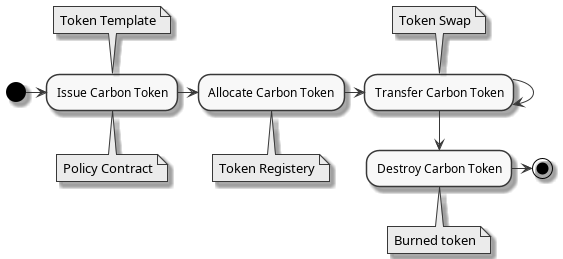
\includegraphics[height=0.2\textwidth, width=0.5\textheight]
        {figures/Token}
    \end{figure}
\end{frame}
\subsection{Energy Producer Accounts}
\begin{frame}{Account Creation}
    \begin{itemize}
        \item Producer creates account, the quantity of energy
              production created by the firm
              is checked on-chain to allocate \textit{Carboncoin}.
        \item Simple heuristic - amount of energy production is recorded
              by a regulator and \textit{Carboncoin} is distributed to
              producers based on the on-chain recording.
        \item \textit{Hyperledger Certificate Authority} generates a
              \textit{X.509} certificate to facilitate blockchain invokes
              for a user.
    \end{itemize}
    \begin{figure}
        \caption{Policy Contract for Token Allocation}
        \centering
        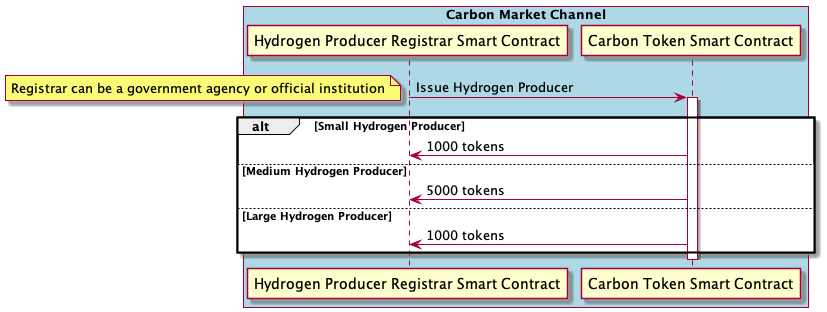
\includegraphics[height=0.3\textwidth, width=0.8\textheight]
        {figures/chain.png}
    \end{figure}
\end{frame}
\begin{frame}{Account Creation Architecture}
    \begin{figure}
        \caption{Account Creation}
        \centering
        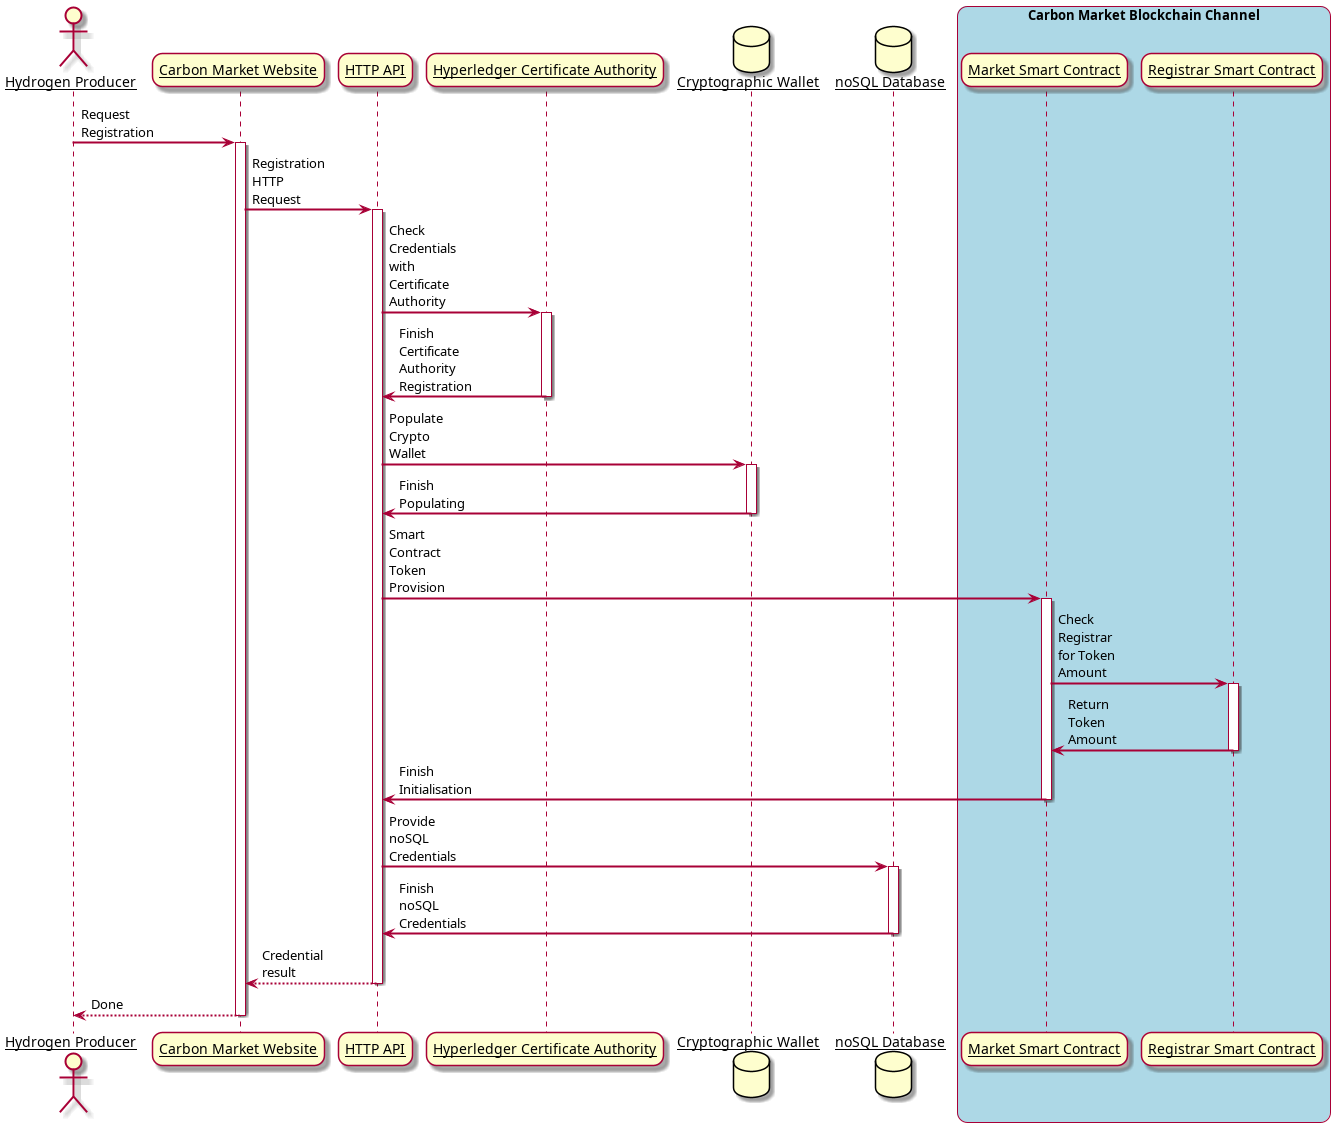
\includegraphics[height=0.6\textheight, width=0.7\linewidth]
        {figures/AccountCreation.png}
    \end{figure}
\end{frame}
\subsection{Carbon Trading}
\begin{frame}{Decentralised Offer Creation}
    \begin{itemize}
        \item Policy contract pattern - requires producer role.
        \item Sale offers constrained by the amount of \textit{Carboncoin}
              in their account minus the quantity they are offering on the open
              market.
        \item Visibility open to all other users.
    \end{itemize}
    \begin{figure}
        \caption{Offer Creation}
        \centering
        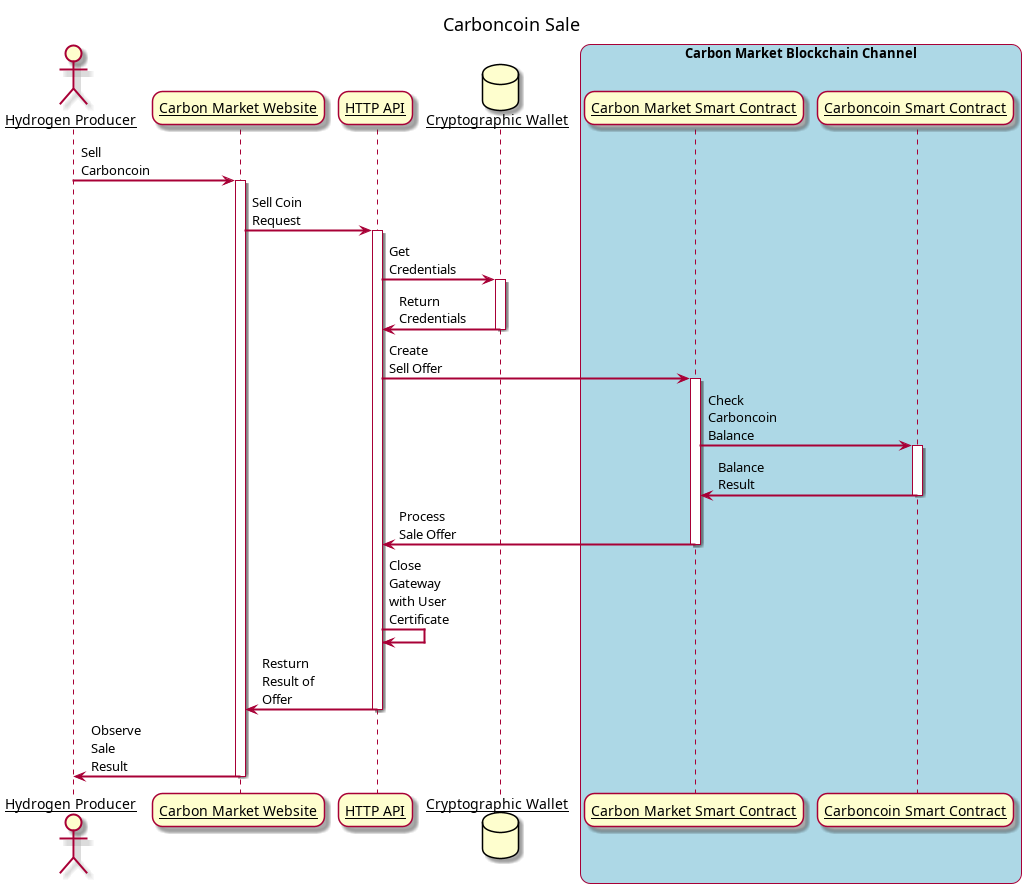
\includegraphics[height=0.4\textheight, width=0.5\linewidth]
        {figures/CreateSale.png}
    \end{figure}
\end{frame}
\begin{frame}{On-chain Order Book}
    \begin{itemize}
        \item On-chain order book.
        \item A template token pattern is utilised to place all
              \textit{Carboncoin} sale offers on-chain.
        \item Generate trust in the market at the expense of chaincode
              performance.
    \end{itemize}
\end{frame}
\begin{frame}{Offer Retrieval}
    \begin{itemize}
        \item Offers are retrieved from an on-chain \textit{couchDB}
              database with a warmed index for performance.
              \begin{figure}
                  \caption{Offer Retrieval}
                  \centering
                  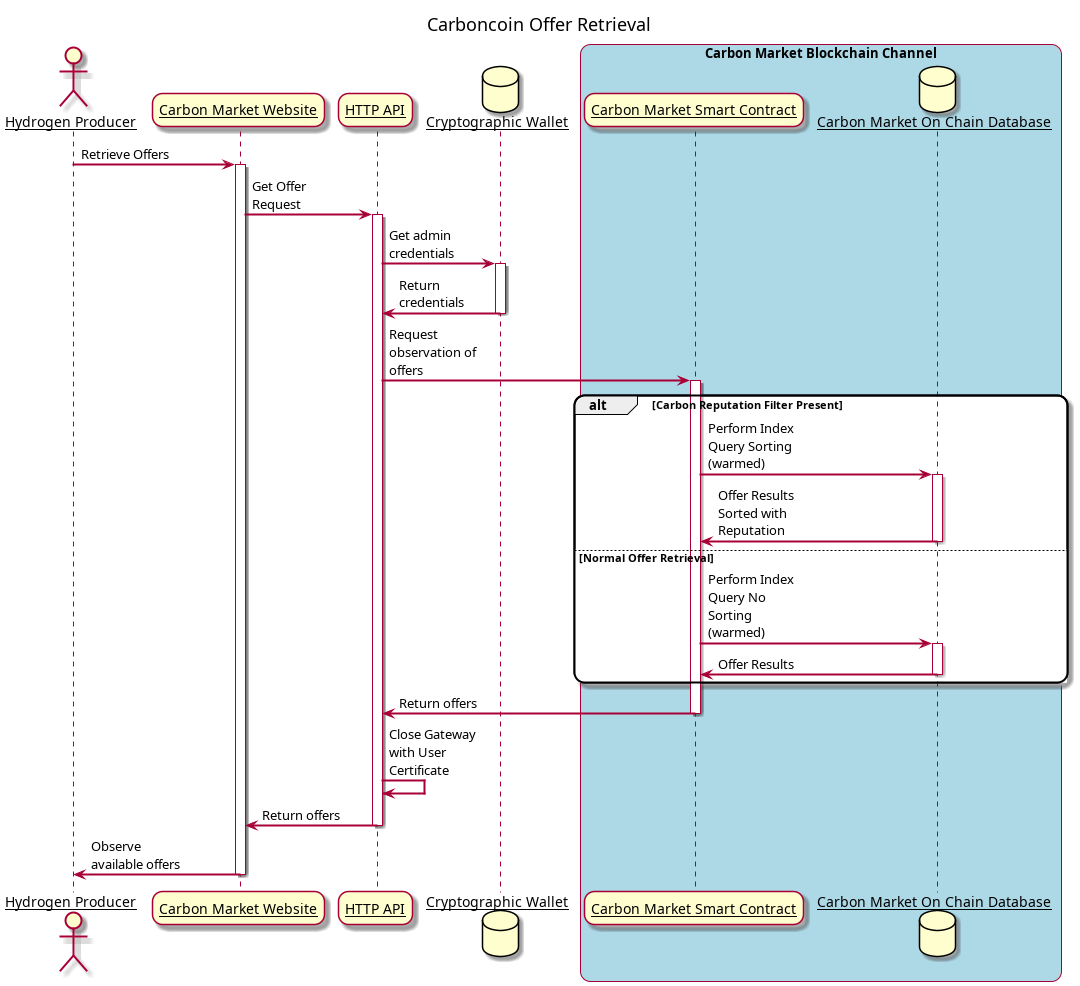
\includegraphics[height=0.5\textheight, width=0.6\textheight]
                  {figures/GetOffersNo.png}
              \end{figure}
    \end{itemize}
\end{frame}
\begin{frame}{Decentralised Sales of Carboncoin}
    \begin{itemize}
        \item Users sell \textit{Carboncoin} - and therefore the right to
              produce emissions to one another - on the open market.
        \item Purpose built offer finder to help users find \textit{Carboncoin}
              to fit a budget.
        \item A token swap pattern is used to facilitate the sale
              of \textit{Carboncoin}.
        \item A sale results in the offerer receiving Australian dollars in
              exchange for \textit{Carboncoin}.
        \item Policy contract attached to chaincode:
              \begin{itemize}
                  \item Active offer is required
                  \item Seller must have enough \textit{Carboncoin}
              \end{itemize}
    \end{itemize}
\end{frame}
\begin{frame}{Sale Architecture}
    \begin{figure}
        \caption{Decentralised Sale}
        \centering
        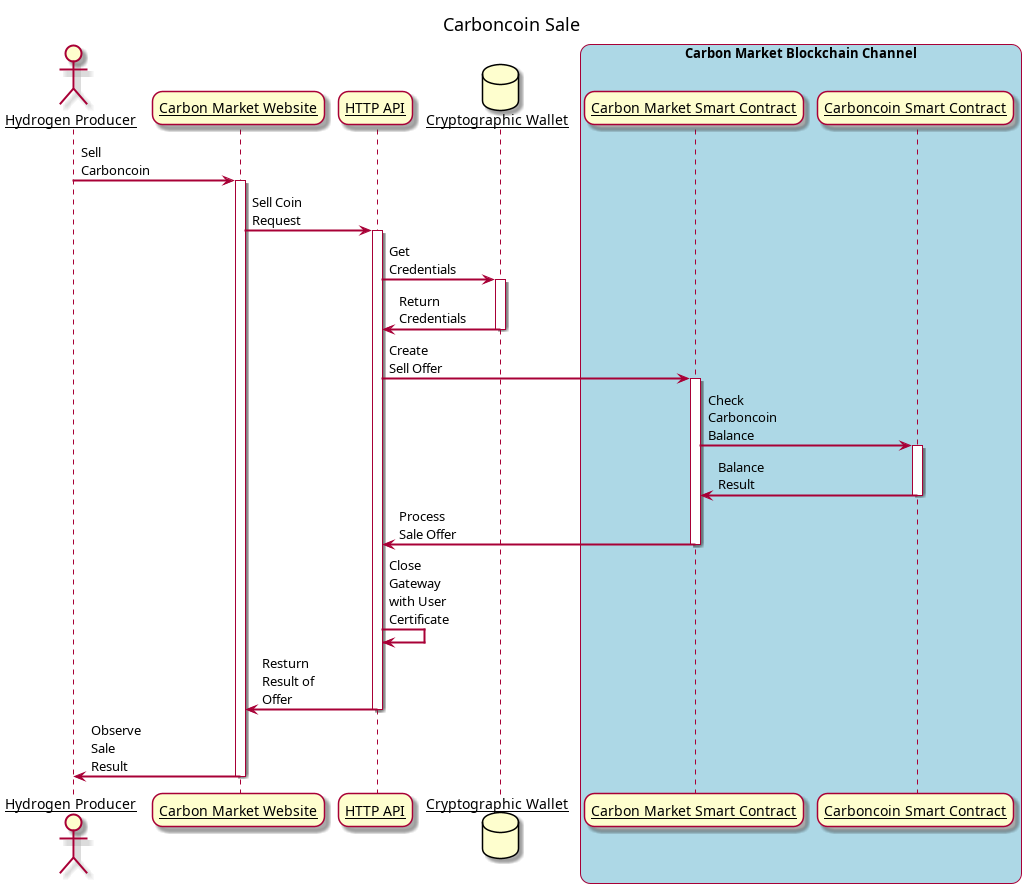
\includegraphics[height=0.7\textheight, width=0.8\textwidth]
        {figures/CreateSale.png}
    \end{figure}
\end{frame}
\begin{frame}{Direct Market Interaction}
    \begin{itemize}
        \item A producer can directly purchase
              \textit{Carboncoin} outside of the open market
              at an \textit{extra cost}.
        \item A policy contract pattern requires the price per
              Carboncoin to reflect a price threshold.
        \item The user is given an on-chain offer token to purchase
              \textit{Carboncoin}.
        \item The price per token is calculated using the maximum offer on the
              open market.
        \item Each $x_i$ in Equation~\ref{eq:1} represents an active offer
              in the market in Australian dollars.
    \end{itemize}
    \begin{equation}
        \text{Direct Offer} =
        \max \left(\left\langle x_1, x_2, \dots, x_n \right\rangle\right) + 50
        \label{eq:1}
    \end{equation}
\end{frame}
\begin{frame}{Direct Offer Creation Example}
    \begin{figure}
        \caption{Direct Offer Creation}
        \centering
        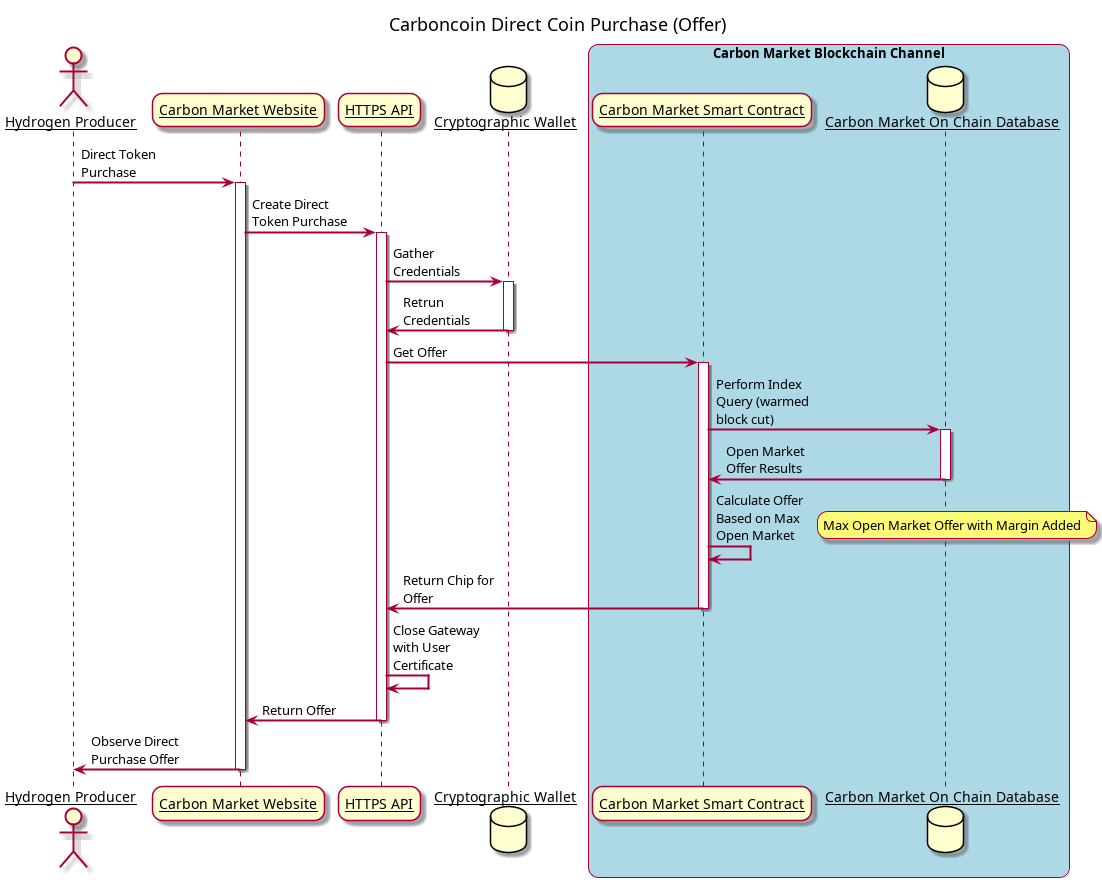
\includegraphics[height=0.7\textheight, width=0.8\textwidth]
        {figures/directOffer.png}
    \end{figure}
\end{frame}
\subsection{ESG Certificate Representation}
\begin{frame}{On-chain ESG Data Compiling}
    \begin{itemize}
        \item Carbon market requires the viewing of Environmental, Social
              and Goverance certificates to automatically expense
              \textit{Carboncoin} and record reputation.
        \item Offload responsibility for on-chain transformation of ESG raw
              data to a useable index onto a `ESG Channel'.
        \item Raw data can be manually/automatically submitted to chaincode
              in the `ESG Channel' which authenticates and verifies to
              produce a final index.
        \item Motivated by recent work from Liu et al in 2021.
    \end{itemize}
\end{frame}
\begin{frame}{ESG Index Compilation Example}
    \begin{figure}
        \caption{ESG Index Compilation}
        \centering
        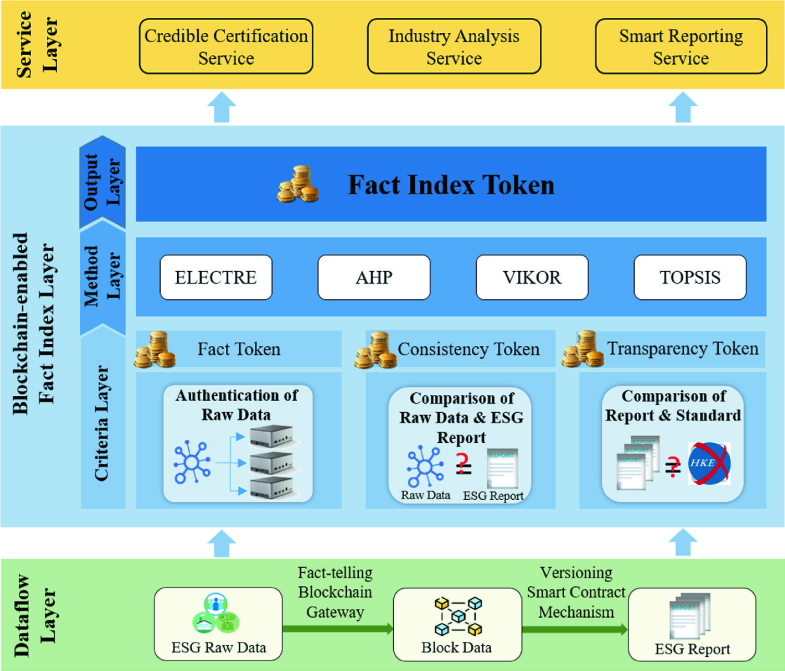
\includegraphics[height=0.6\textheight, width=0.7\textwidth]
        {figures/esg-rep.png}
    \end{figure}
\end{frame}
\subsection{ESG Integration into Market}
\begin{frame}{ESG Integration}
    \begin{itemize}
        \item A carbon market regulator specifies unique weights for
              each ESG category used by energy producers.
        \item As an example, energy production as carbon dioxide
              equivalence is given a negative weight of one whilst good
              quality water used in production is given a score
              of positive two.
        \item The carbon market can weight ESG data outside of the
              environment - such as the female employee rate found
              inside a company's Annual Report.
        \item The baseline weight is for carbon dioxide equivalence (CO2e), it
              always has a weight of negative one reputation.
    \end{itemize}
\end{frame}
\begin{frame}{ESG Integration Architecture}
    \begin{itemize}
        \item The carbon market has specific chaincode to handle
              the `ESG Channel' compiling an index for a market
              participant.
        \item Chaincode applies a weight specified by the regulator
              to provide to the \textit{Carbonmarket} smart contract.
              \begin{figure}
                  \caption{ESG Architecture Interaction}
                  \centering
                  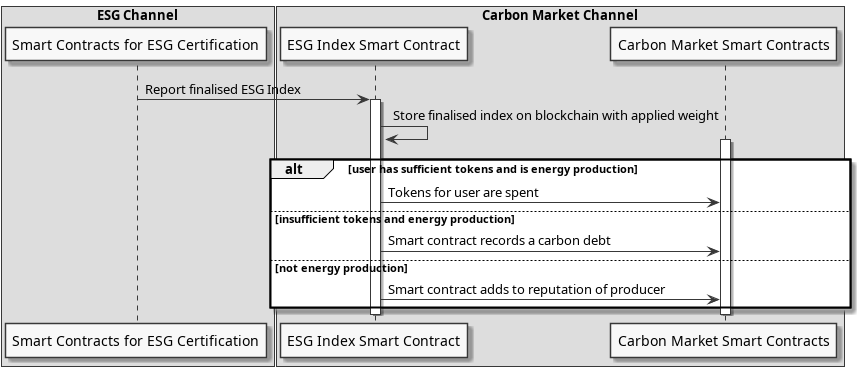
\includegraphics[height=0.4\textheight, width=0.7\textwidth]
                  {figures/reputation.png}
              \end{figure}
    \end{itemize}
\end{frame}
\begin{frame}{Automated ESG Reputation}
    \begin{itemize}
        \item The carbon market smart contract uses the weighted index
              score to generate a reputation breakdown for all energy producers
              on the platform.
        \item Can be viewed mathematically as a weighted sum - where each
              $x_i$ is an ESG index value and $w_i$ is a weight for the index
              category $x_i$ in Equation~\ref{eq:2}. Applied to all $n$
              ESG index scores for a producer.
        \item Once added the reputation is persistent.
        \item Reputation is automatically updated for each user when a new
              ESG index is made in the `ESG Channel'.
    \end{itemize}
    \begin{equation}
        \text{Reputation} = \sum_{i=1}^{n}x_i \cdot w_i
        \label{eq:2}
    \end{equation}
\end{frame}
\begin{frame}{Reputation Blockchain Patterns}
    \begin{itemize}
        \item Token template - each ESG index instantiates a token template
              with fields for the original statistic, weight and reputation
              breakdown.
        \item Policy contract - reputation can only be added by the `ESG Index
              Smart Contract' on the Carbon Market Channel.
        \item Access control - reputation breakdown is viewable for each
              user with the producer role in the system.
    \end{itemize}
\end{frame}